% Auto-generated by experiments.analysis.generate_win_counts --slides --- do not edit.
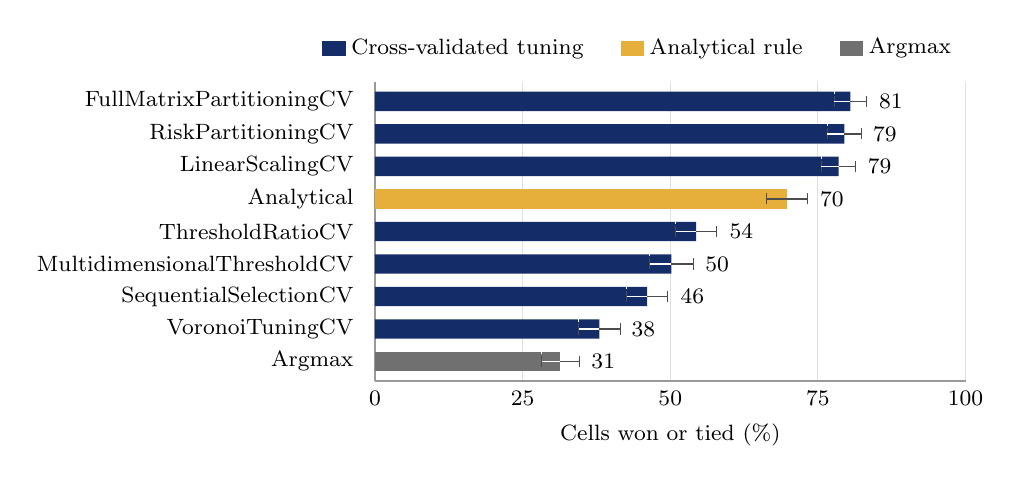
\begin{tikzpicture}
\definecolor{winbarcv}{HTML}{142D69}
\definecolor{winbarsplit}{HTML}{7FB6E6}
\definecolor{winbaranalytical}{HTML}{E6AF3C}
\definecolor{winbarargmax}{HTML}{707070}
\begin{axis}[
    xbar, bar shift=0pt, bar width=7pt,
    scale only axis, width=7.5cm, height=3.80cm,
    xmin=0, xmax=100, xtick={0,25,50,75,100},
    xlabel={Cells won or tied (\%)},
    ymin=0.4, ymax=9.6, y dir=reverse,
    ytick={1,2,3,4,5,6,7,8,9},
    yticklabels={FullMatrixPartitioningCV,RiskPartitioningCV,LinearScalingCV,Analytical,ThresholdRatioCV,MultidimensionalThresholdCV,SequentialSelectionCV,VoronoiTuningCV,Argmax},
    axis x line*=bottom, axis y line*=left,
    axis line style={draw=black!40},
    tick style={draw=none},
    xmajorgrids=true,
    major grid style={draw=black!12, line width=0.3pt},
    tick label style={font=\footnotesize},
    label style={font=\footnotesize},
    clip=false,
    legend columns=3,
    legend cell align=left,
    legend image code/.code={\fill[#1] (0cm,-0.1cm) rectangle (0.3cm,0.1cm);},
    legend style={draw=none, fill=none, font=\footnotesize,
        at={(1,1.04)}, anchor=south east,
        /tikz/every even column/.append style={column sep=0.4cm}},
]
\addplot[fill=winbarcv, draw=none, error bars/x dir=both, error bars/x explicit, error bars/error bar style={black!70, line width=0.5pt}] coordinates { (80.5,1) +- (2.7,0) (79.5,2) +- (2.9,0) (78.5,3) +- (2.9,0) (54.4,5) +- (3.5,0) (50.2,6) +- (3.7,0) (46.1,7) +- (3.5,0) (38.0,8) +- (3.5,0) };
\addlegendentry{Cross-validated tuning}
\addplot[fill=winbaranalytical, draw=none, error bars/x dir=both, error bars/x explicit, error bars/error bar style={black!70, line width=0.5pt}] coordinates { (69.8,4) +- (3.5,0) };
\addlegendentry{Analytical rule}
\addplot[fill=winbarargmax, draw=none, error bars/x dir=both, error bars/x explicit, error bars/error bar style={black!70, line width=0.5pt}] coordinates { (31.4,9) +- (3.2,0) };
\addlegendentry{Argmax}
\draw[white, line width=0.5pt] (axis cs:80.5,1) -- (axis cs:77.8,1) +(0,-2pt) -- +(0,2pt);
\draw[white, line width=0.5pt] (axis cs:79.5,2) -- (axis cs:76.6,2) +(0,-2pt) -- +(0,2pt);
\draw[white, line width=0.5pt] (axis cs:78.5,3) -- (axis cs:75.6,3) +(0,-2pt) -- +(0,2pt);
\draw[white, line width=0.5pt] (axis cs:54.4,5) -- (axis cs:50.9,5) +(0,-2pt) -- +(0,2pt);
\draw[white, line width=0.5pt] (axis cs:50.2,6) -- (axis cs:46.5,6) +(0,-2pt) -- +(0,2pt);
\draw[white, line width=0.5pt] (axis cs:46.1,7) -- (axis cs:42.6,7) +(0,-2pt) -- +(0,2pt);
\draw[white, line width=0.5pt] (axis cs:38.0,8) -- (axis cs:34.5,8) +(0,-2pt) -- +(0,2pt);
\draw[white, line width=0.5pt] (axis cs:31.4,9) -- (axis cs:28.2,9) +(0,-2pt) -- +(0,2pt);
\node[anchor=west, font=\footnotesize, inner sep=1pt] at (axis cs:84.8,1) {81};
\node[anchor=west, font=\footnotesize, inner sep=1pt] at (axis cs:83.8,2) {79};
\node[anchor=west, font=\footnotesize, inner sep=1pt] at (axis cs:82.9,3) {79};
\node[anchor=west, font=\footnotesize, inner sep=1pt] at (axis cs:74.8,4) {70};
\node[anchor=west, font=\footnotesize, inner sep=1pt] at (axis cs:59.5,5) {54};
\node[anchor=west, font=\footnotesize, inner sep=1pt] at (axis cs:55.4,6) {50};
\node[anchor=west, font=\footnotesize, inner sep=1pt] at (axis cs:51.2,7) {46};
\node[anchor=west, font=\footnotesize, inner sep=1pt] at (axis cs:42.9,8) {38};
\node[anchor=west, font=\footnotesize, inner sep=1pt] at (axis cs:36.1,9) {31};
\end{axis}
\end{tikzpicture}%
